% Copyright 2004 by Till Tantau <tantau@users.sourceforge.net>.
%
% In principle, this file can be redistributed and/or modified under
% the terms of the GNU Public License, version 2.
%
% However, this file is supposed to be a template to be modified
% for your own needs. For this reason, if you use this file as a
% template and not specifically distribute it as part of a another
% package/program, I grant the extra permission to freely copy and
% modify this file as you see fit and even to delete this copyright
% notice. 

\documentclass{beamer}

% There are many different themes available for Beamer. A comprehensive
% list with examples is given here:
% http://deic.uab.es/~iblanes/beamer_gallery/index_by_theme.html
% You can uncomment the themes below if you would like to use a different
% one:
%\usetheme{AnnArbor}
%\usetheme{Antibes}
%\usetheme{Bergen}
%\usetheme{Berkeley}
%\usetheme{Berlin}
%\usetheme{Boadilla}
%\usetheme{boxes}
%\usetheme{CambridgeUS}
%\usetheme{Copenhagen}
%\usetheme{Darmstadt}
%\usetheme{default}
%\usetheme{Frankfurt}
%\usetheme{Goettingen}
%\usetheme{Hannover}
%\usetheme{Ilmenau}
%\usetheme{JuanLesPins}
%\usetheme{Luebeck}
\usetheme{Madrid}
%\usetheme{Malmoe}
%\usetheme{Marburg}
%\usetheme{Montpellier}
%\usetheme{PaloAlto}
%\usetheme{Pittsburgh}
%\usetheme{Rochester}
%\usetheme{Singapore}
%\usetheme{Szeged}
%\usetheme{Warsaw}


\usepackage{graphicx}
\newcommand{\shellcmd}[1]{\\\indent\indent\texttt{\footnotesize\# #1}\\}  %For linux commands

\title{Getting Started}

% A subtitle is optional and this may be deleted
\subtitle{Session 1}

%\author{F.~Author\inst{1} \and S.~Another\inst{2}}
% - Give the names in the same order as the appear in the paper.
% - Use the \inst{?} command only if the authors have different
%   affiliation.

\institute[Computer Vision Group] % (optional, but mostly needed)
{
  Computer Vision Group\\
  IIT Madras
%  \and
%  \inst{2}%
%  Department of Theoretical Philosophy\\
%  University of Elsewhere}
% - Use the \inst command only if there are several affiliations.
% - Keep it simple, no one is interested in your street address.
}
\date{November 1, 2014}
% - Either use conference name or its abbreviation.
% - Not really informative to the audience, more for people (including
%   yourself) who are reading the slides online

\subject{Theoretical Computer Science}
% This is only inserted into the PDF information catalog. Can be left
% out. 

% If you have a file called "university-logo-filename.xxx", where xxx
% is a graphic format that can be processed by latex or pdflatex,
% resp., then you can add a logo as follows:

% \pgfdeclareimage[height=0.5cm]{university-logo}{university-logo-filename}
% \logo{\pgfuseimage{university-logo}}

% Delete this, if you do not want the table of contents to pop up at
% the beginning of each subsection:
%\AtBeginSubsection[]
%{
%  \begin{frame}<beamer>{Outline}
%    \tableofcontents[currentsection,currentsubsection]
%  \end{frame}
%}

% Let's get started
\begin{document}

\begin{frame}
  \titlepage
\end{frame}

\begin{frame}{Outline}
  \tableofcontents
  % You might wish to add the option [pausesections]
\end{frame}

% Section and subsections will appear in the presentation overview
% and table of contents.
\section{Installation OpenCV}

\subsection{Windows}

\begin{frame}{Installing OpenCV}{Windows 7/8}
  \begin{itemize}
  \item {
    Install Anaconda 2.0.1
  }
  \item {
    Download OpenCV 2.4.9 and extract to a convenient location
  }
  \item{
    Go to opencv/build/python/2.7 folder
  }
  \item{
    Copy cv2.pyd to INSTALL\_DIRECTORY/Python/lib/site-packages
  }
  \item{
    Open IPython QT console.
  }
  \item{
    import cv2
  }
  \end{itemize}
  If you don't get any errors, its a success.
\end{frame}

\subsection{Ubuntu}

% You can reveal the parts of a slide one at a time
% with the \pause command:
\begin{frame}{Installing OpenCV}{Ubuntu}
\begin{block}{Using the apt-get tool}
sudo apt-get install python-opencv
\end{block}

%  \item {   
%    Second item.
%  }
  % You can also specify when the content should appear
  % by using <n->:
%  \item<3-> {
%    Third item.
%  }
%  \item<4-> {
%    Fourth item.
%  }
  % or you can use the \uncover command to reveal general
  % content (not just \items):
%  \item<5-> {
%    Fifth item. \uncover<6->{Extra text in the fifth item.}
%  }

Installs an older version of OpenCV. Build from source to get the latest version.
\end{frame}


\section{Concepts in Image Processing}
\subsection{Pixels}

\begin{frame}{Pixels}{Recap}
\centering
    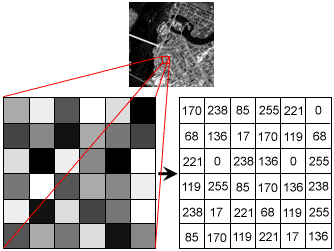
\includegraphics[width=50mm]{images/pixel.png} 

\begin{itemize}
\item Basic building blocks of an image
\item Color represented as a tuple (R, G, B)
\end{itemize}
\end{frame}

\subsection{Image Processing}
\begin{frame}{Image Processing}{Recap}
\begin{itemize}
\item Thresholding
\pause
\item Erosion
\pause
\item Dilation
\end{itemize}
\end{frame}

\subsection{Image Transformations}
\begin{frame}{Image Transformations}{Recap}
\begin{itemize}
\item Rotation
\pause
\item Translation
\pause
\item Cropping
\pause
\item Warping
\end{itemize}
\end{frame}

\section{Feature Extraction}
\subsection{What are features?}
\begin{frame}{Feature Extraction}{What are features?}
\begin{block}{Feature Extraction in Images}
Transforming rich content of images into a set of values. Feature extraction is a crucial part in Machine Learning.
%TODO Improve this
\end{block}
\pause
\begin{example}
Histograms are commonly used for extracting set of features. More feature extraction techniques coming up.
\end{example}

\pause
\begin{block}{Digit Recognizer}
We'll be using Machine Learning to build a digit recognizer in tomorrow's session. 
\end{block}

\end{frame}

\subsection{Why we need feature extraction?}
\begin{frame}{Feature Extraction}{Why we need features?}
Lets say you are in an unkown country. 
To know about the country, you can see each and every house in it, and using the reference information about all houses (location and shape) in every country, you can find which country you are in.
That sounds bad, lets take an helicopter and fly. What you can see now are not houses, but streets filled with houses. You now have a feature set of smaller size (All street names in the country) which you can use to deduce the country.
Even that can be difficult, so you can fly further up and now you see cities, which should make the task fairly easy.
It is the same case with feature extraction. You look at the dataset from a higher abstraction, extract relevant features (like City names) and train your machine.
The catch here is you cannot fly so high that you see the country as a whole to directly find what it is. Using whatever abstraction possible (Similar to city names), you try to learn higher levels of abstraction (Country names).
\end{frame}

\subsection{Some feature extraction tools}
\begin{frame}{Feature Extraction Tools}{There are many more available}
\begin{enumerate}
\item Binarized pixel values
\pause
\item Intensity histogram
\pause
\item Histogram of Oriented gradients
\pause
\item SIFT
\end{enumerate}
\end{frame}



% Placing a * after \section means it will not show in the
% outline or table of contents.
\section*{Summary}
\begin{frame}{Summary}

\begin{block}{Today's session}
\begin{itemize}
\item Image processing/transformations
\item Feature Extraction
\end{itemize}
\end{block}

\begin{block}{Tomorrow's session}
\begin{itemize}
\item Machine Learning Basics
\item Training a classifier for handwritten digit recognition
\end{itemize}
\end{block}




\end{frame}


\end{document}
